\section{Results}

\subsection{Image processing}
\label{sec:image_processing}

To show how the processing was done, two images will be used as examples. One will be used as the reference image (figure \ref{fig:001_background}), and the other will contain an object to be analysed (figure \ref{fig:002_blue_cap}). These two images will then be sent through the process in figure \ref{fig:image_visualization_program_flow} with a noise limit of 10. 

The results from the processing are the two images in figure \ref{fig:hadamard_division_blue_cap}. They have been normalized and multiplied with 255 so that it is easy to see the changes. %TODO Are they actually histogram equalized? I don't really think so, I just normalized them and multiplied with 255.
Figure \ref{fig:002_blue_cap_positive_difference} shows what colors in what pixels have gotten more light after the blue cap was introduced. On the other hand figure \ref{fig:002_blue_cap_negative_difference} shows the colors that have gotten weaker after introducing the cap. What this means will be discussed further in section \ref{sec:blue_cap_discussion}

\begin{figure}[h]
    \begin{subfigure}{0.5\textwidth}
        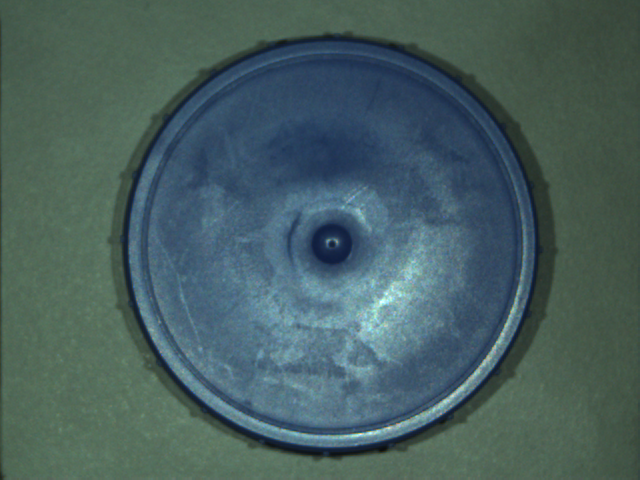
\includegraphics[width=0.9\linewidth, height=5cm]{figures/camera_pictures_png/002_blue_cap.png}
        \caption{002 Blue cap, $A$}
        \label{fig:002_blue_cap}
    \end{subfigure}%
    \begin{subfigure}{0.5\textwidth}
        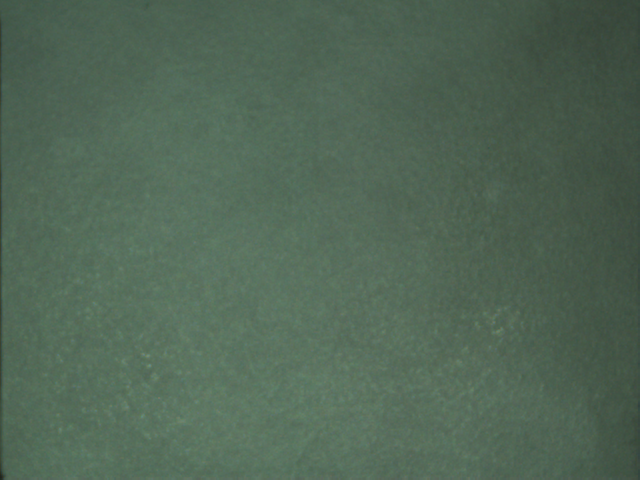
\includegraphics[width=0.9\linewidth, height=5cm]{figures/camera_pictures_png/001_background.png}
        \caption{001 Background, $A_0$}
        \label{fig:001_background}
    \end{subfigure}
    
    \caption{The original images being used in figure \ref{fig:hadamard_division_blue_cap}}
    \label{fig:blue_cap_and_background}
\end{figure}

\begin{figure}[h]
        \begin{subfigure}{0.5\textwidth}
            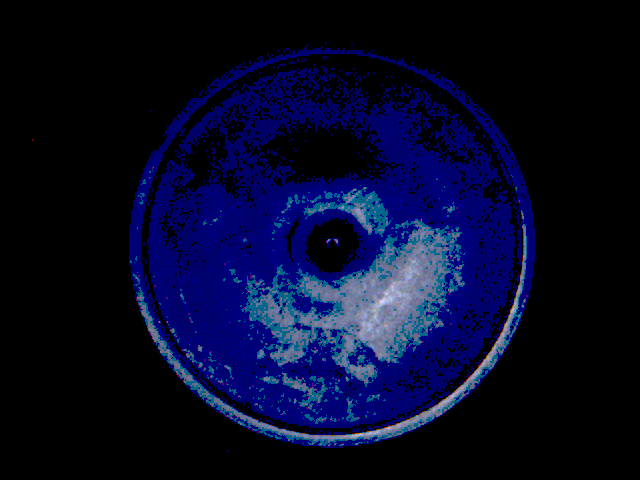
\includegraphics[width=0.9\linewidth, height=5cm]{figures/processed_camera_pictures/002_blue_cap_positive_difference.png}
            \caption{$RR'_{positive}$}
            \label{fig:002_blue_cap_positive_difference}
        \end{subfigure}%
        \begin{subfigure}{0.5\textwidth}
            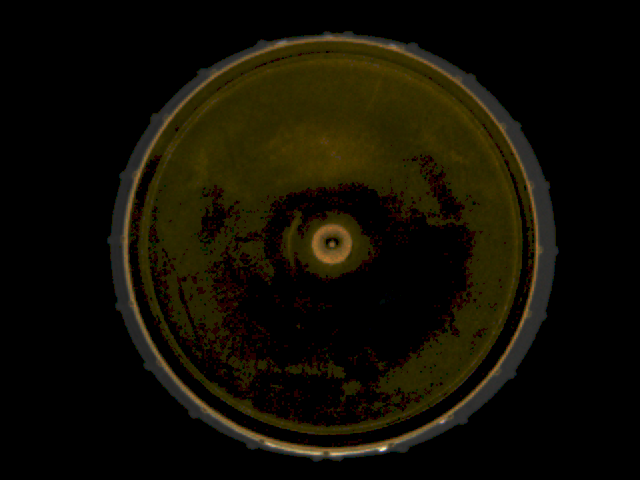
\includegraphics[width=0.9\linewidth, height=5cm]{figures/processed_camera_pictures/002_blue_cap_negative_difference.png} 
            \caption{$RR'_{negative}$}
            \label{fig:002_blue_cap_negative_difference}
    \end{subfigure}
    
    \caption{Hadamard division for the blue cap}
    \label{fig:hadamard_division_blue_cap}
\end{figure}

\subsection{Spectrum processing}

The spectrum was analysed in a similar manner, but here it was not necessary for the sake of visualization to split it into two results. It was however needed to subtract 1 from the results so that it was easy to compare the spectrums before and after multiplying with QE to each other (\ref{eq:relative_reflectance_minus_one}). It also helped for comparison with the image. 
The recorded spectrums for the reference image and the blue cap are shown in figure \ref{fig:blue_cap_and_reference_spectrum}. The black line is the reference background spectrum, and the blue line is the line when the blue cap is introduced. 

\begin{figure}[h]
    \centering
    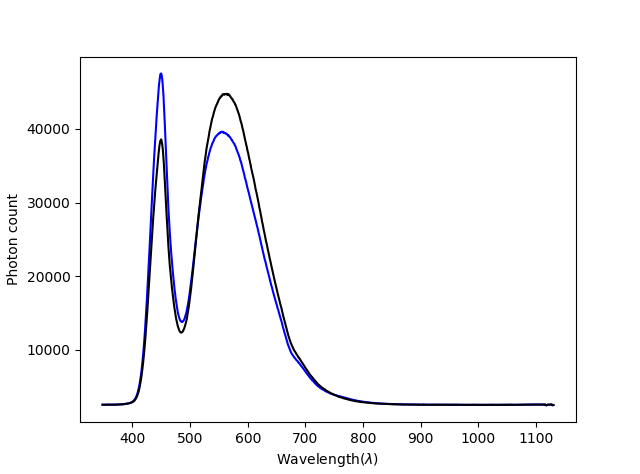
\includegraphics[width=0.75\textwidth]{Plots/blue_cap_original_spectrum_and_background.png}
    \caption{Comparison of blue cap (blue) and reference specter (black)}
    \label{fig:blue_cap_and_reference_spectrum}
\end{figure}

\begin{figure}[h]
    \centering
    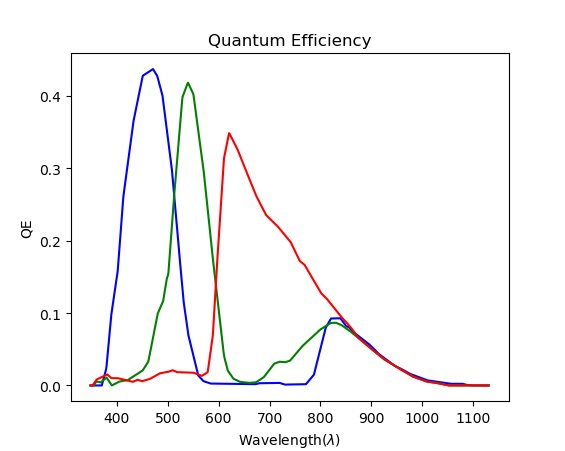
\includegraphics[width=0.75\textwidth]{Plots/quantum_effiency.png}
    \caption{The quantum efficiency of the camera Bayer mask}
    \label{fig:quantum_efficiency_camera}
\end{figure}


Figure \ref{fig:blue_cap_spectrum} shows relative reflectance minus one for the blue cap. It also includes the spectrums that the camera "sees" for each color, i.e. the wavelength parts and their respective magnitudes that is taken in by the CCD sensor. They are shown in their original colors; blue, green and red. The quantum efficiency used is shown in figure \ref{fig:quantum_efficiency_camera}. 

\begin{figure}[h]
    \centering
    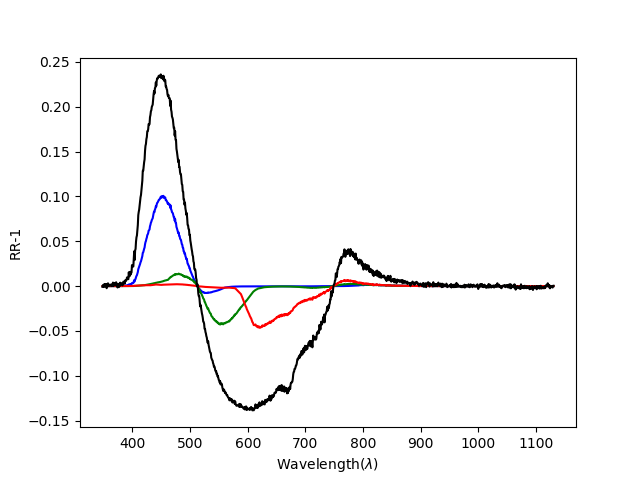
\includegraphics[width=0.75\textwidth]{Plots/blue_cap_rr_minus_one_with_qe.png}    
    \caption{Spectrum of blue cap}
    \label{fig:blue_cap_spectrum}
\end{figure}


\subsection{Ideal situation}
\label{sec:ideal_situation}
30 images and spectrums where run through the software and the spectral and spatial average value was compared to each other. In figure \ref{fig:spectral_vs_spatial_values} the spatial and spectral averages are plotted against each other, together with three linear regression lines. The blue line shows the regression line used for correlating the spatial and spectral average of the blue pixels. The red line shows the regression line for the red color, and lastly the green line shows the regression line for the green color. These 30 images where taken under the best conditions that could be made in the lab, with the minimum amount of noise. This set will be used as basis for comparison with images taken with one unideal pertubation. 

\begin{figure}[h]
    \centering
    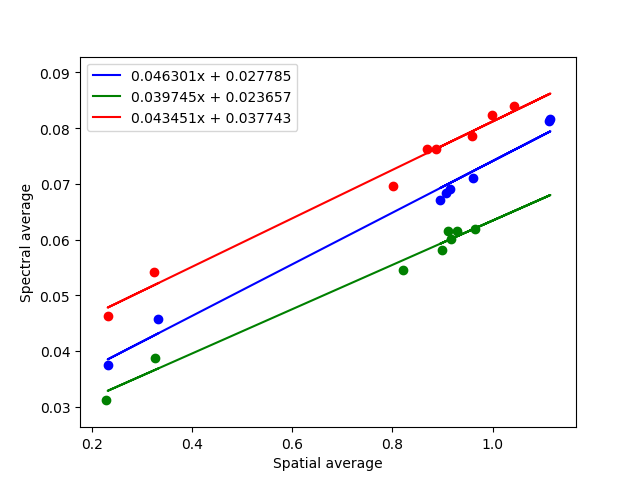
\includegraphics[width=0.75\textwidth]{Plots/spectral_vs_spatial_average_with_regression.png}
    \caption{Spatial and spectral averages plotted against each other with the fitted regression lines}
    \label{fig:spectral_vs_spatial_values}
\end{figure}

\subsection{Pertubation}
To see how well the value can be used for testing correspondence between image and spectrum, several images where taken that show unideal situations. These images where made with 10 randomly chosen settings from the ideal case, but with some unideal pertubation. They will be compared to the regression lines created in section \ref{sec:ideal_situation} with the error function. 

For both the ideal and unideal cases the average error and variance of the error compared to the regression line was calculated and is presented in \ref{tb:error_estimate}.

\begin{table}[h]
    \centering
    \caption{Estimated error of the regression lines}
    \label{tb:error_estimate}
    \begin{tabular}{@{}llllllll@{}}
    \toprule
                   &                 & \multicolumn{3}{l}{Error average} & \multicolumn{3}{l}{Error variance} \\ \midrule
    Situation      & \#              & Blue       & Green     & Red      & Blue       & Green     & Red       \\
    Ideal          & 30              & 0.001261   & 0.001229  & 0.001370 & 6.744e-07  & 5.384e-07 & 8.963e-07 \\
    Ambient light  & 10              & 0.001805   & 0.001544  & 0.002349 & 1.860e-06  & 2.488e-06 & 1.016e-06 \\
    Border object  & 10              & 0.0007057  & 0.0005739 & 0.001615 & 6.581e-07  & 2.114e-07 & 6.382e-07 \\
    Outside object & 10              & 0.0006382  & 0.0009339 & 0.002476 & 1.174e-07  & 1.430e-07 & 1.876e-07 \\ \bottomrule
    \end{tabular}
\end{table}


\textbf{Ambient light}
These images where taken without turning of the light in the room. And with a fluorescent stand lamp on pointing towards the measurement area. Figure \ref{fig:ambient_light_plot} shows how these data points compare to the regression lines made in the ideal situation.

\begin{figure}[h]
    \centering
    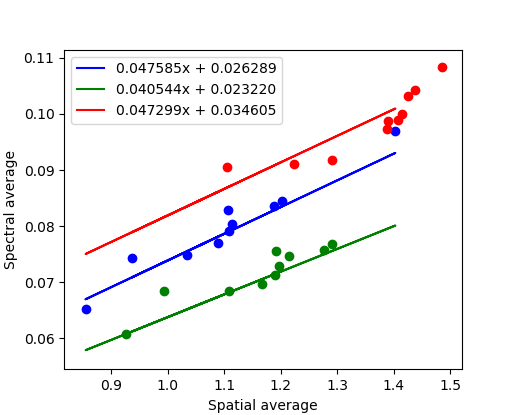
\includegraphics[width=0.5\textwidth]{Plots/spectral_vs_spatial_average_with_regression_ambient_light.png}
    \caption{Ambient light data points compared to ideal regression line}
    \label{fig:ambient_light_plot}
\end{figure}

\textbf{Border of imaging area}
Objects where put so that they where only partly inside the imaging area, but could still be seen by the spectrometer. Figure \ref{fig:boundary_objects_plot} shows how these data points compare to the regression lines made in the ideal situation.

\begin{figure}[h]
    \centering
    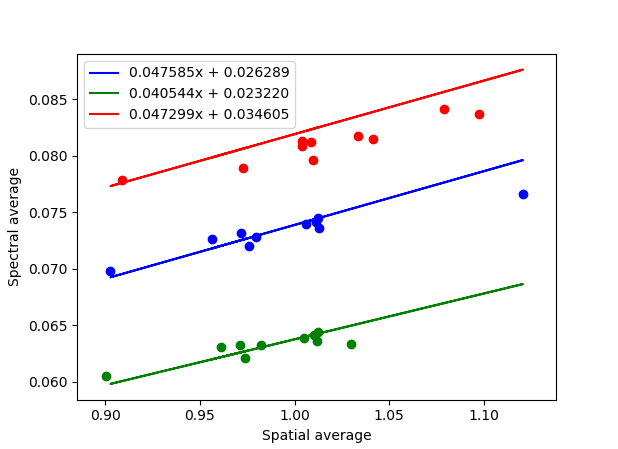
\includegraphics[width=0.5\textwidth]{Plots/spectral_vs_spatial_average_with_regression_boundary_objects.png}
    \caption{Objects placed on the boundary}
    \label{fig:boundary_objects_plot}
\end{figure}

\textbf{Outside the imaging area}
The same object where put inside the cameras viewpoint for every image, but a different object where put just outside it. It should still be inside the spectrometers view angle. Figure \ref{fig:outside_objects_plot} shows how these data points compare to the regression lines made in the ideal situation.

\begin{figure}[h]
    \centering
    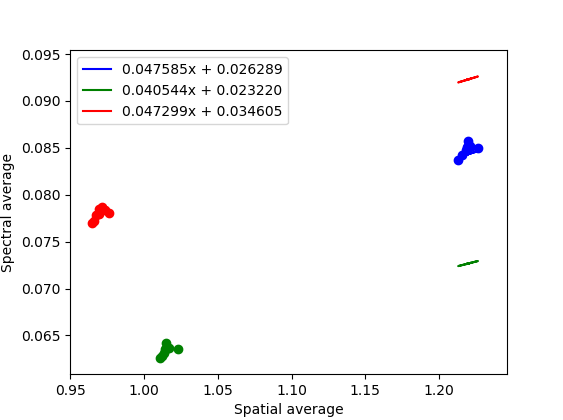
\includegraphics[width=0.5\textwidth]{Plots/spectral_vs_spatial_average_with_regression_outside_objects.png}
    \caption{One object inside boundary, another outside}
    \label{fig:outside_objects_plot}
\end{figure}

%\subsection{Specular reflection}

\section{Discussion}
The spatial and spectral average should be two sides of the same story, if the camera and the spectrometer are watching the same area and the conditions haven't changed between the camera taking the picture and the spectrometer taking the spectre. The purpose of taking these results where to test this postulate that was originally stated in section \ref{sec:introduction}.

\subsection{Blue cap}
\label{sec:blue_cap_discussion}

In section \ref{sec:image_processing} the image of a Blue cap vs a reference background image was analysed. 
Figure \ref{fig:002_blue_cap_positive_difference} shows the pixels that have had an increase in pixel color value after the blue cap was introduced. Blue is the dominant color here, but there are also some spots that have a strong white color. This is due to the difference between specular and diffusive reflection presented in section \ref{sec:theory_reflection}. 

Specular reflection reflects in the same direction and will for that reason give a stronger signal than diffusive when it hits the camera. It will however only hit if the angle between the light source, the object and the camera is very specific. It is because of the strong reflection that it appears white, all three of the color sensors have reached their limit and is given out the maximum value. Specular reflection will only appear in the $RR'_{positive}$ image. 

For more diffusive parts however the light is spread in several directions and the return value to the camera is therefore weaker and it is not normal to over expose these reflections. Diffusive reflectance shows up in both $RR'_{positive}$ and $RR'_{negative}$. It is what gives us the most color to work with. 


Figure \ref{fig:spectral_vs_spatial_values} shows the results from 30 pictures taken under ideal conditions. The lines shown in blue, green and red are regression lines (sec \ref{sec:regression}) that are made as a minimum variance fit to the points. It looks like each of the color sensors have approximately the same number $a$, meaning that they have similar derivatives, but different $b$ means that they cross the y axis at different points. 

The error measurement given in table \ref{tb:error_estimate} shows the amount of error in the different situations. From the table we can see that the ambient light is the type of noise that is creating the most variance from the regression line. The other measurements actually show less variance which was not expected, but probably means that the acceptance cone of the spectrometer was smaller than expected, and not any bigger than the cameras acceptance cone. 

\textbf{Ambient light}
From the results it can be inferred that the light sources where the most important in this setup. Having ambient light on made the error increase to almost twice the previous error. This can be due to: 
\begin{itemize}
    \item More shadows are formed because light comes from other directions. 
    \item The reference picture without ambient light is very different to an image with ambient light. 
    \item The overhead lamp has many spikes in its spectrum, which could be a source of noise. 
\end{itemize}


\textbf{Border of the imaging area} and \textbf{Outside the image area}
Both of these led to smaller error than the ideal situation, which is strange. It can be due to the acceptance cone being much smaller than assumed, leading to changes outside of the black box not making any difference. This combined with the smaller change between image and reference due to the objects being placed on the border could explain the smaller error. 

\textbf{Shadows}
Part of the reason that parts of the wavelength gets weaker when an object is introduced is due to shadows. If the light doesn't come from the same fiber that is also receiving the light, an object with depth will cast a shadow. The image will get affected by this and in figure \ref{fig:002_blue_cap_negative_difference} you can see a darker white around the cork. Due to using two light sources it doesn't become a complete shadow. It should be possible to recognize the shadow with image processing and remove it. For the spectrum the shadow will decrease the amplitude of the resultant spectrum, but since the shadow effectively means that the light intensity is halved for all wavelengths this shouldn't affect the form of the spectrum. The reason it should be halved is that in our images one of the two light sources have always been able to light up every point. A shadow in this case is therefore when one light source is blocked. With more heterogenous materials both light sources can be blocked. This will not be addressed here.



The effects of the dark current \ref{sec:noise_and_dark_current} was hopefully minimized by finding the relative reflectance and introducing the noise limit into the image processing. 